\documentclass[a4paper,11pt]{article}
\pdfoutput=1 % if your are submitting a pdflatex (i.e. if you have
             % images in pdf, png or jpg format)

\usepackage{jinstpub} % for details on the use of the package, please
                      % see the JINST-author-manual


\usepackage[english, russian]{babel}  % <- удалить после перевода!!!!!!!!!!!!!!!!!!!!!!!!!!
\usepackage[utf8]{inputenc}           % <- удалить после перевода!!!!!!!!!!!!!!!!!!!!!!!!!!



\title{\boldmath Investigation of energy spectrum and chemical composition of primary cosmic rays in 1--100 PeV energy range with a drone-borne installation}

%% %simple case: 2 authors, same institution
%% \author{A. Uthor}
%% \author{and A. Nother Author}
%% \affiliation{Institution,\\Address, Country}

% more complex case: 4 authors, 3 institutions, 2 footnotes
\author[a,1]{D.~Chernov,\note{Corresponding author.}}
\author[a]{E.~Bonvech,}
\author[c,d]{M.~Finger~Jr.,}
\author[c,d]{M.~Finger,}
\author[b]{V.~Galkin,}
\author[b]{V.~Ivanov,}
\author[a,b]{D.~Podgrudkov,}
\author[a]{T.~Roganova,}
\author[a,b]{I.~Vaiman}

% The "\note" macro will give a warning: "Ignoring empty anchor..."
% you can safely ignore it.

\affiliation[a]{Lomonosov Moscow State University, Skobeltsyn Institute for Nuclear Physics, Moscow, Russian Federation}
\affiliation[b]{Lomonosov Moscow State University, Faculty of Physics, Moscow, Russian Federation}
\affiliation[c]{Charles University, Faculty of Mathematics and Physics, Prague, Czech Republic}
\affiliation[d]{Joint Institute for Nuclear Research, Dubna, Russian Federation}

% e-mail addresses: only for the corresponding author
\emailAdd{chr@dec1.sinp.msu.ru}


\abstract{This work is dedicated to the development of a project aimed at the implementation of a relatively new method of studying the PCR --- the registration of optical Vavilov-Cherenkov radiation, often called “Cherenkov light”, from EAS (EAS CL), reflected from the snow surface. The objective of the project is to create an installation for the study of the cosmic ray mass composition in the energy range of 1--100 PeV by detecting the reflected EAS CL. Silicon photomultipliers are planned to be used in the detector of the installation, and an unmanned aerial vehicle (UAV, drone) will be used to lift the measuring equipment over the snow-covered surface.}


\keywords{Cherenkov detectors, Mass spectrometers, Balloon instrumentation.}


%\arxivnumber{1234.56789} % only if you have one


% \collaboration{\includegraphics[height=17mm]{example-image}\\[6pt]
%   XXX collaboration}
% or
%\collaboration[c]{on behalf of XXX collaboration}


% if you write for a special issue this may be useful
\proceeding{Instrumentation for Colliding Beam Physics, INSTR20\\
from 24 to 28 February, 2020\\
Novosibirsk, Russia}



\begin{document}
\maketitle
\flushbottom

\section{Introduction}
\label{sec:intro}

The  1--100 PeV energy range is transitional from galactic to extragalactic cosmic rays. More than 50 years ago a change in the slope of the energy spectrum of primary cosmic rays (PCR) was detected at around 3 PeV. But until now new features in the structure of the spectrum are being discovered. In this regard it is interesting to understand the cause of these slope irregularities. The main reason, most likely, are changes in the mass composition of the PCR. Presently used methods allow to estimate either the average mass of PCR particles or to divide them into ``light''' and ``heavy'' groups. Basically, estimates are made on the reconstructed depth of development maximum of the extensive air showers (EAS), using the the modelling of the shower development in the atmosphere. Since the methodological uncertainties of the reconstructed parameters mass groups can be identified only by processing a large amount of experimental data.

The project is aimed at development of a unique detector using modern photodetectors based on silicon photomultipliers (SiPM), which is installed on an unmanned aerial vehicle. Currently, there are no other devices and installations that would successfully use reflected Cherenkov light registration method. The method allows to achieve the highest accuracy of estimation of the chemical composition of PCR in the analysis of the individual EAS events in comparison with existing ground installations. The successful implementation of the project will allow obtaining experimental data for the reconstruction of partial spectra for several mass groups of PCR particles (protons, helium, CNO and Fe groups) in the 1--100 PeV energy range.



\begin{figure}[htbp]
\centering
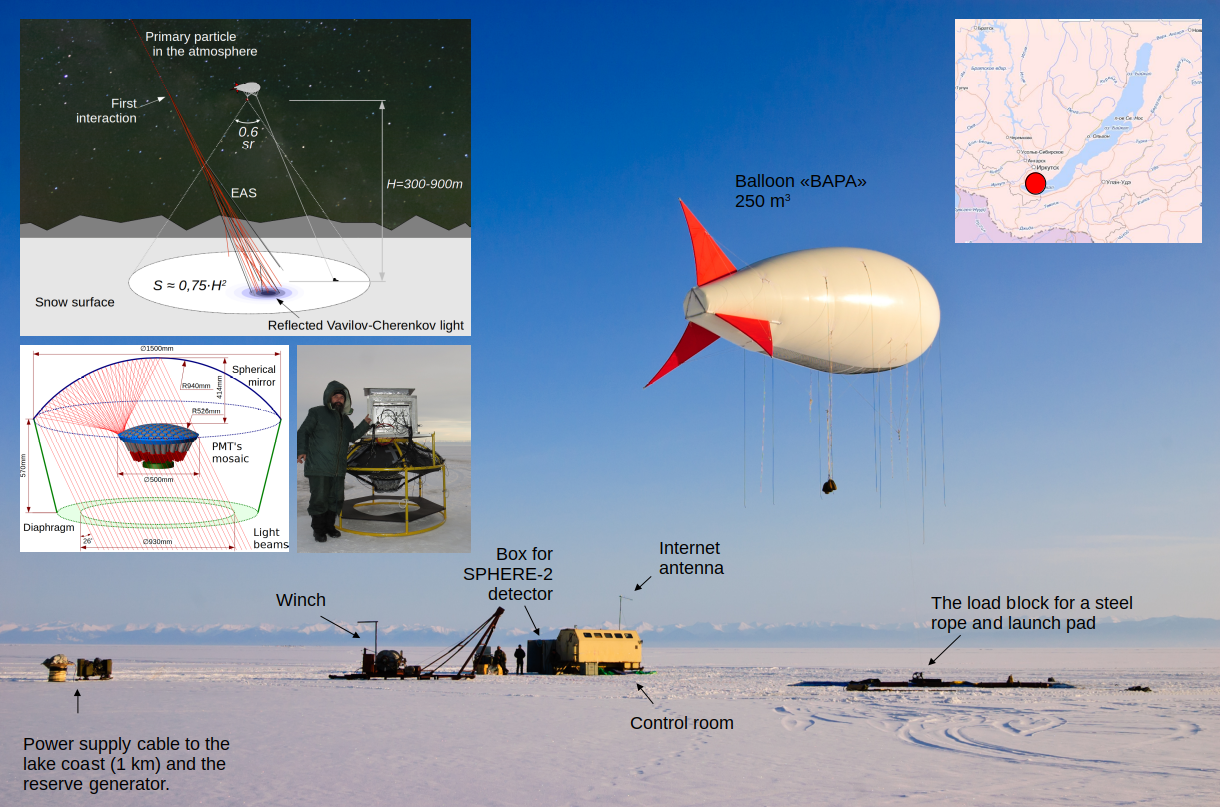
\includegraphics[width=.8\textwidth,trim=0 0 0 0,clip]{Sphere2Baikal.png}
\caption{\label{fig:1} Experiment with the SPHERE-2 installation on lake Baikal.}
\end{figure}


\section{Previous work}

We propose to apply a new unique tecnique to cosmic rays study. The main idea of this experiment consists in the detection of the extensive air showers Cherenkov light reflected from the snowed earth surface with the compact apparatus lifted above the earth. The technique was verified in our earlier experiments~\cite{1,2}.

In the period from 2008 to 2013, a series of measurements of reflected Cherenkov light was carried out using the SPHERE-2~\cite{1,2,3} balloon detector. Measurements were made on the snow-covered ice of Baikal lake. The Figure~\ref{fig:1} shows the landing point

The energy spectrum of all particles was measured. And the light nuclei part estimation~\ref{fig:2} was calculated. The results was published in~\cite{2}. 

\begin{figure}[htbp]
\centering % \begin{center}/\end{center} takes some additional vertical space
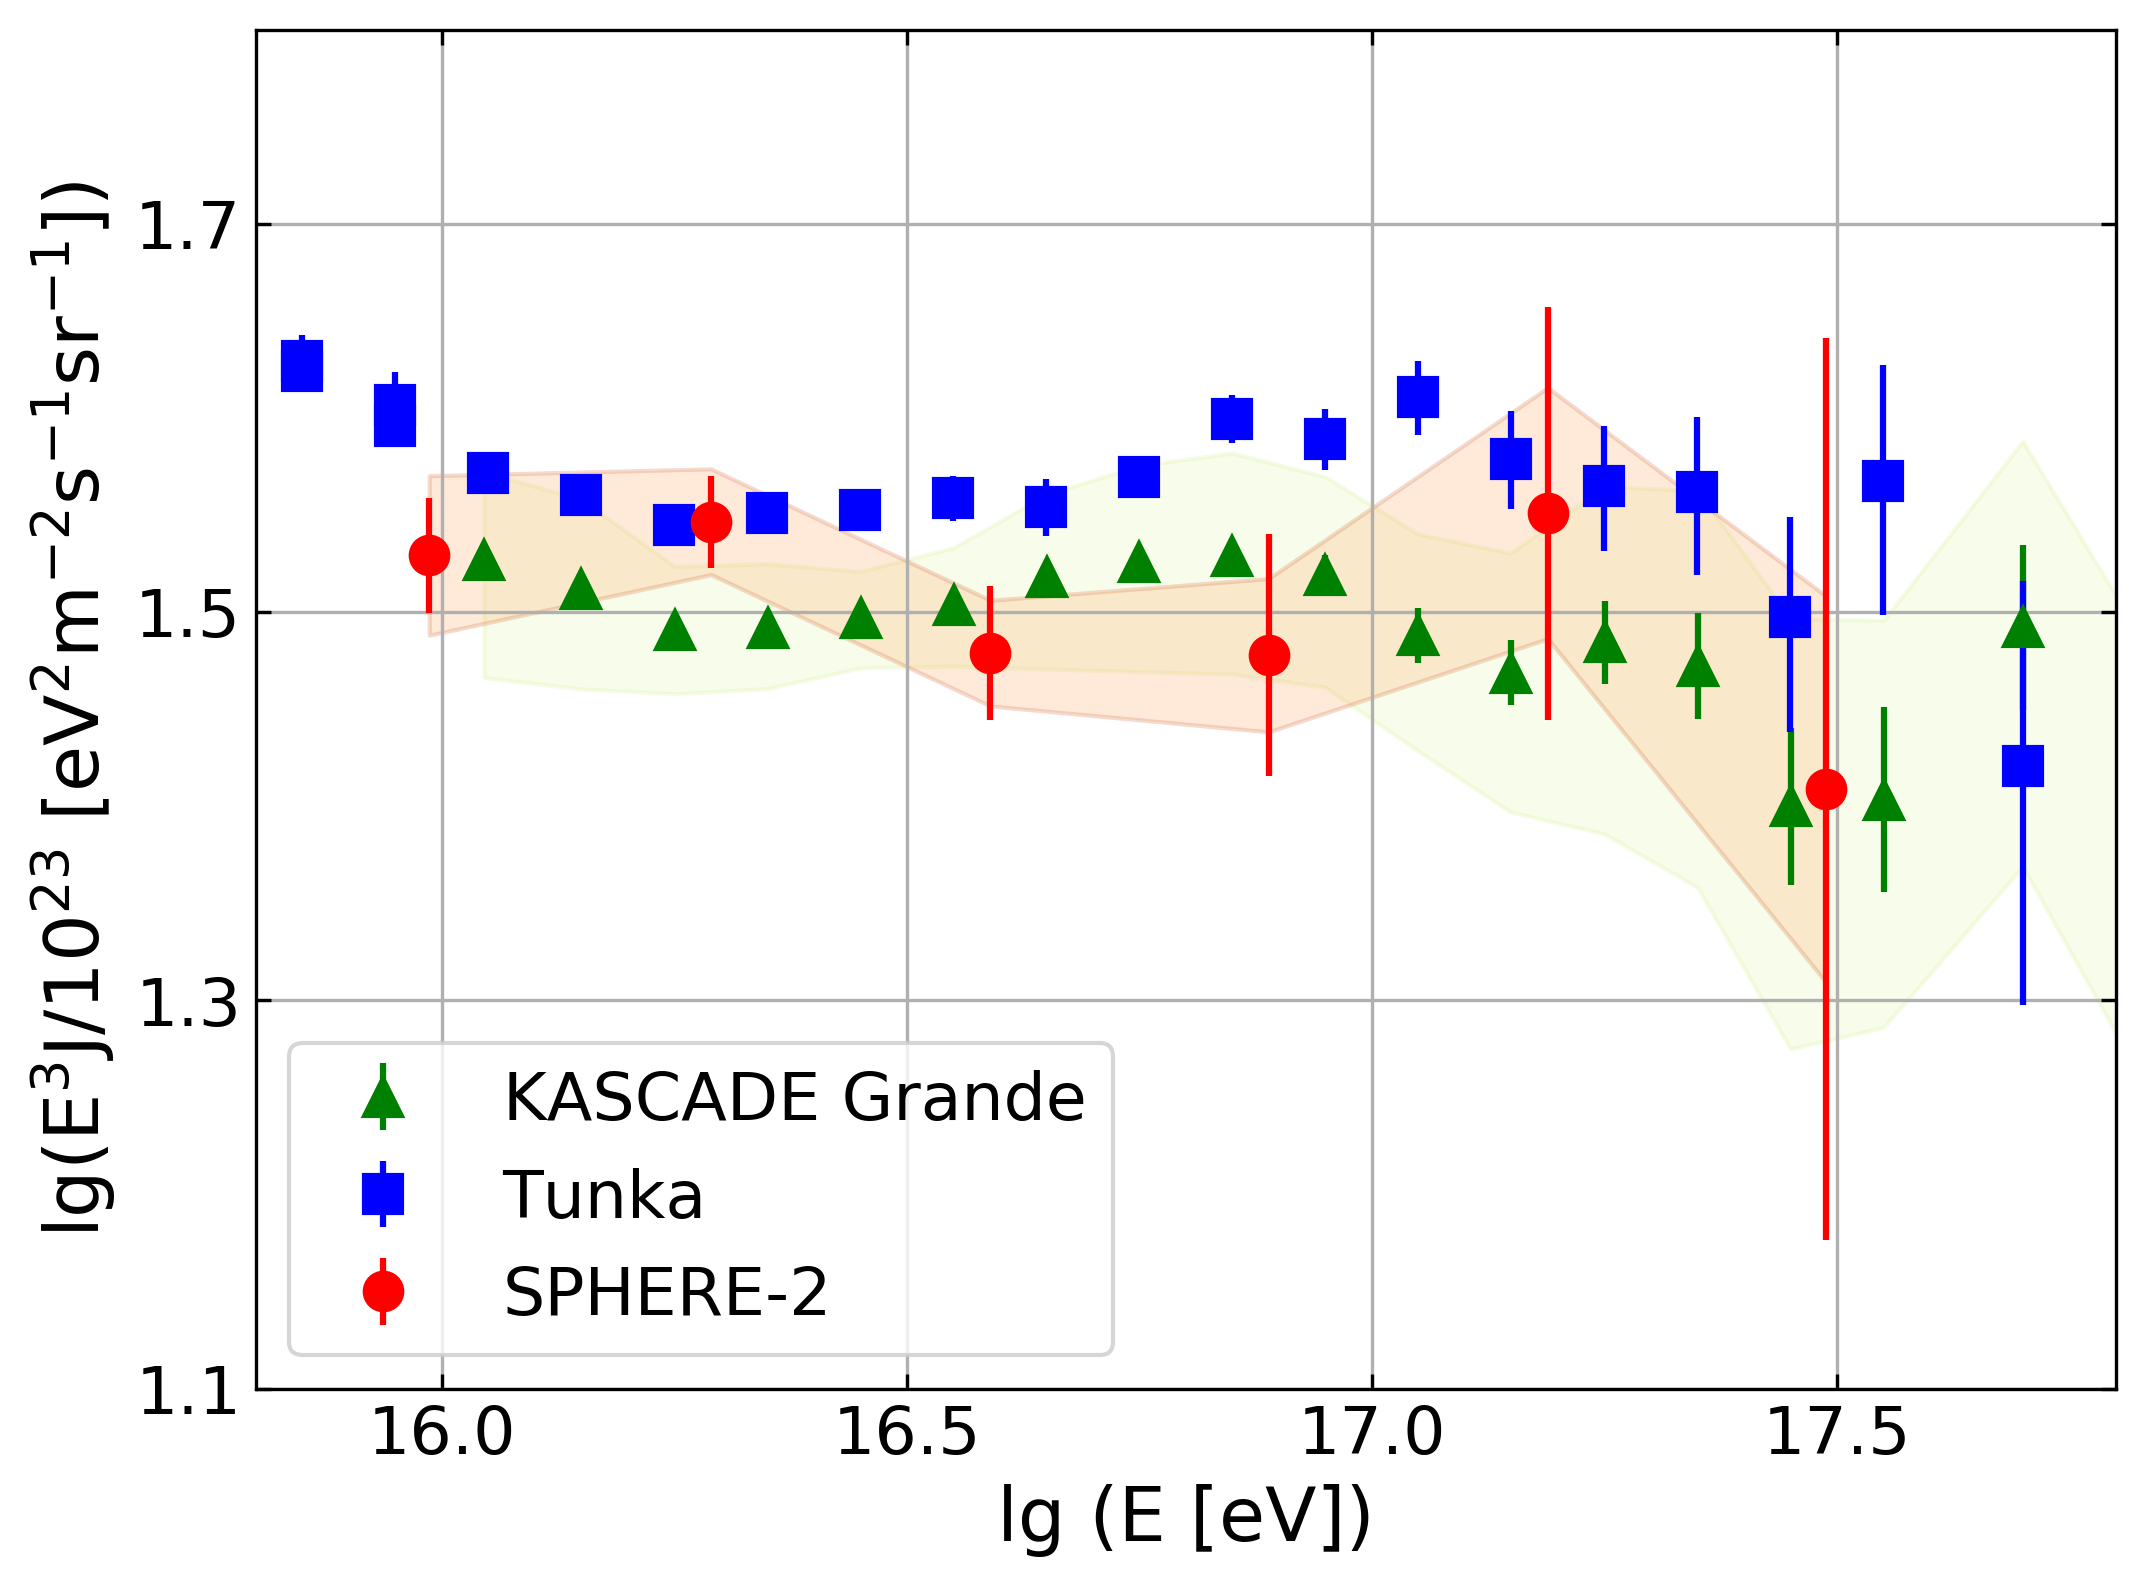
\includegraphics[width=.4\textwidth,trim=0 0 0 0,clip]{sphere2spectrum.png}
\qquad
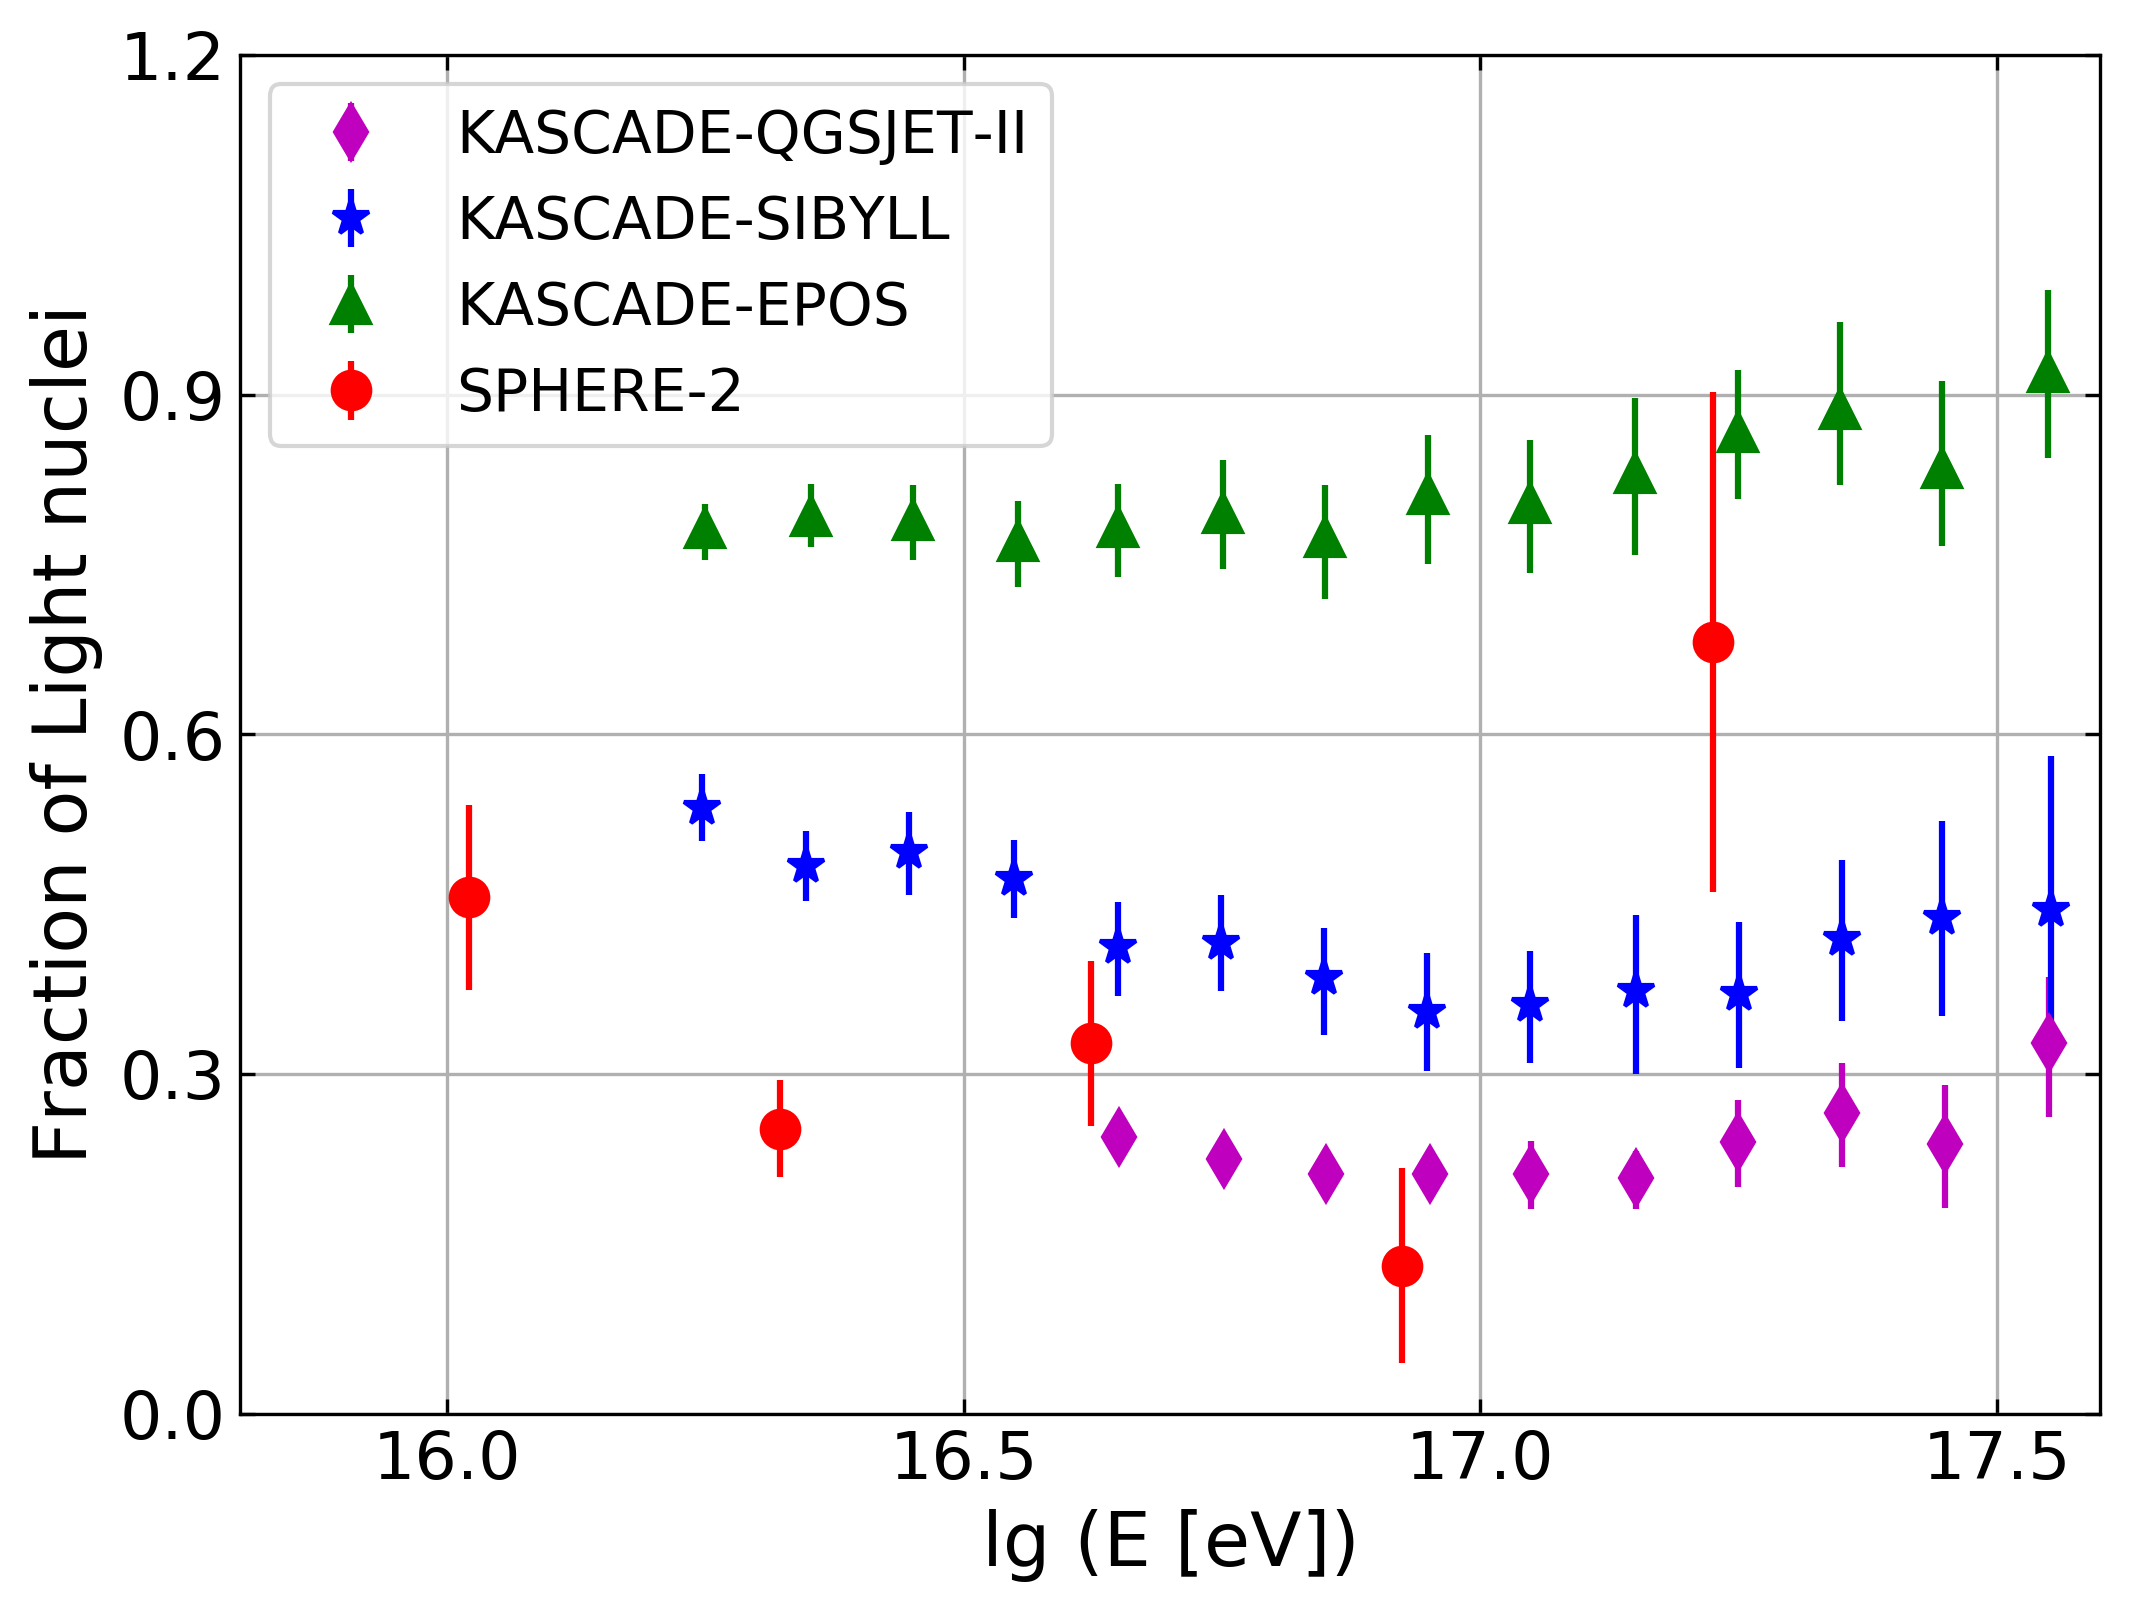
\includegraphics[width=.4\textwidth,origin=c,angle=0]{sphere2composition.png}
% "\includegraphics" from the "graphicx" permits to crop (trim+clip)
% and rotate (angle) and image (and much more)
\caption{\label{fig:2} Results of previous work with the SPHERE-2 installation. Energy spectrum (left) and chemical composition estimates (right).}
\end{figure}





\section{Advantages of the method}

\begin{itemize}
\item Provides a significant area of CL registration using a compact device;
\item Accurate estimation of PCR energy in an individual event in comparison with other methods;
\item The field of view of the individual sensitive elements of the device covers a significant part of the surveyed area, which allows observation the CL from EAS near the shower axis, usually inaccessible to ground-based CL detector arrays. This circumstance significantly increases the accuracy of the primary particle type estimation;
\item Allows measurement of the same PCR energy range with different resolution (distance between the centres of the fields of view of neighbouring sensing elements) using variation of the detector elevation, which allows you to control the magnitude of systematic errors.
\end{itemize}


\section{Detector}


\begin{figure}[htbp]
\centering % \begin{center}/\end{center} takes some additional vertical space
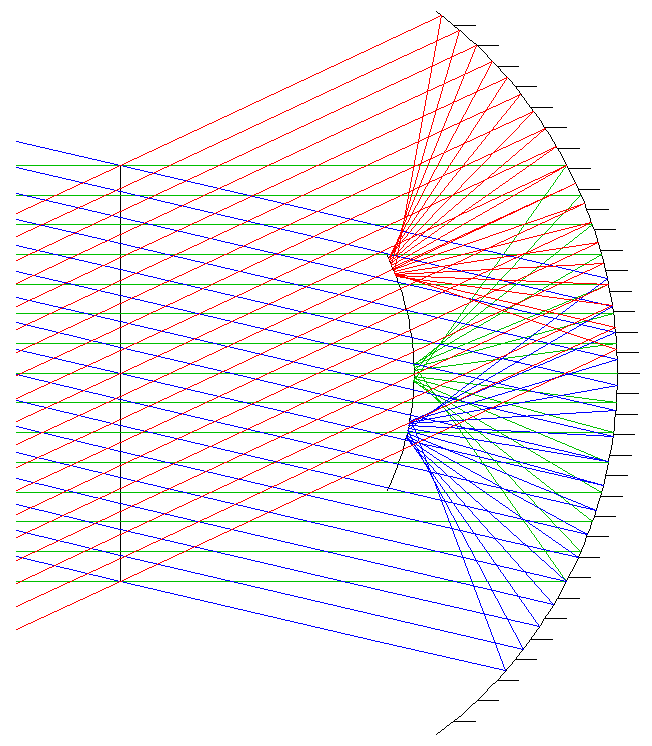
\includegraphics[width=.32\textwidth,clip]{Sphere3optic.png}
\qquad
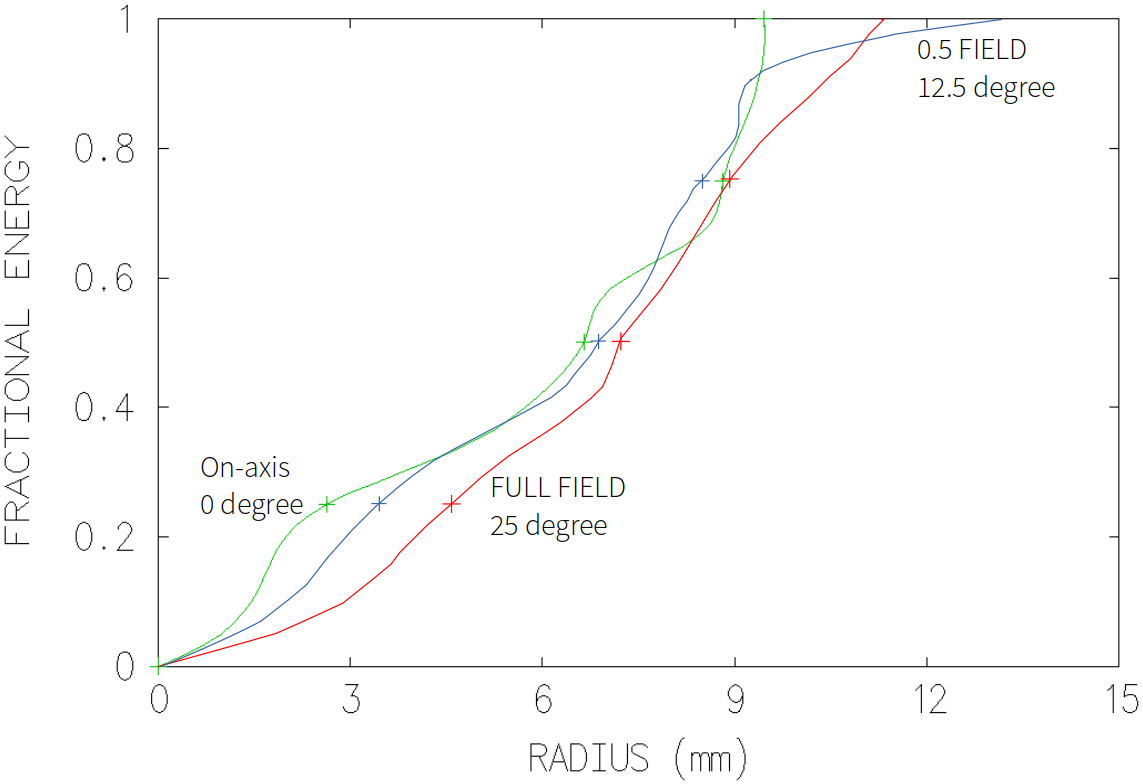
\includegraphics[width=.48\textwidth,origin=c,angle=0]{Sphere3spot_energy.png}
% "\includegraphics" from the "graphicx" permits to crop (trim+clip)
% and rotate (angle) and image (and much more)
\caption{\label{fig:sphere3} Optical scheme of the developed detector (without shadow of the mosaic) and the fractional light energy distribution on focal plane taking into account the shadow from the mosaic.}
\end{figure}


\begin{figure}[htbp]
\centering
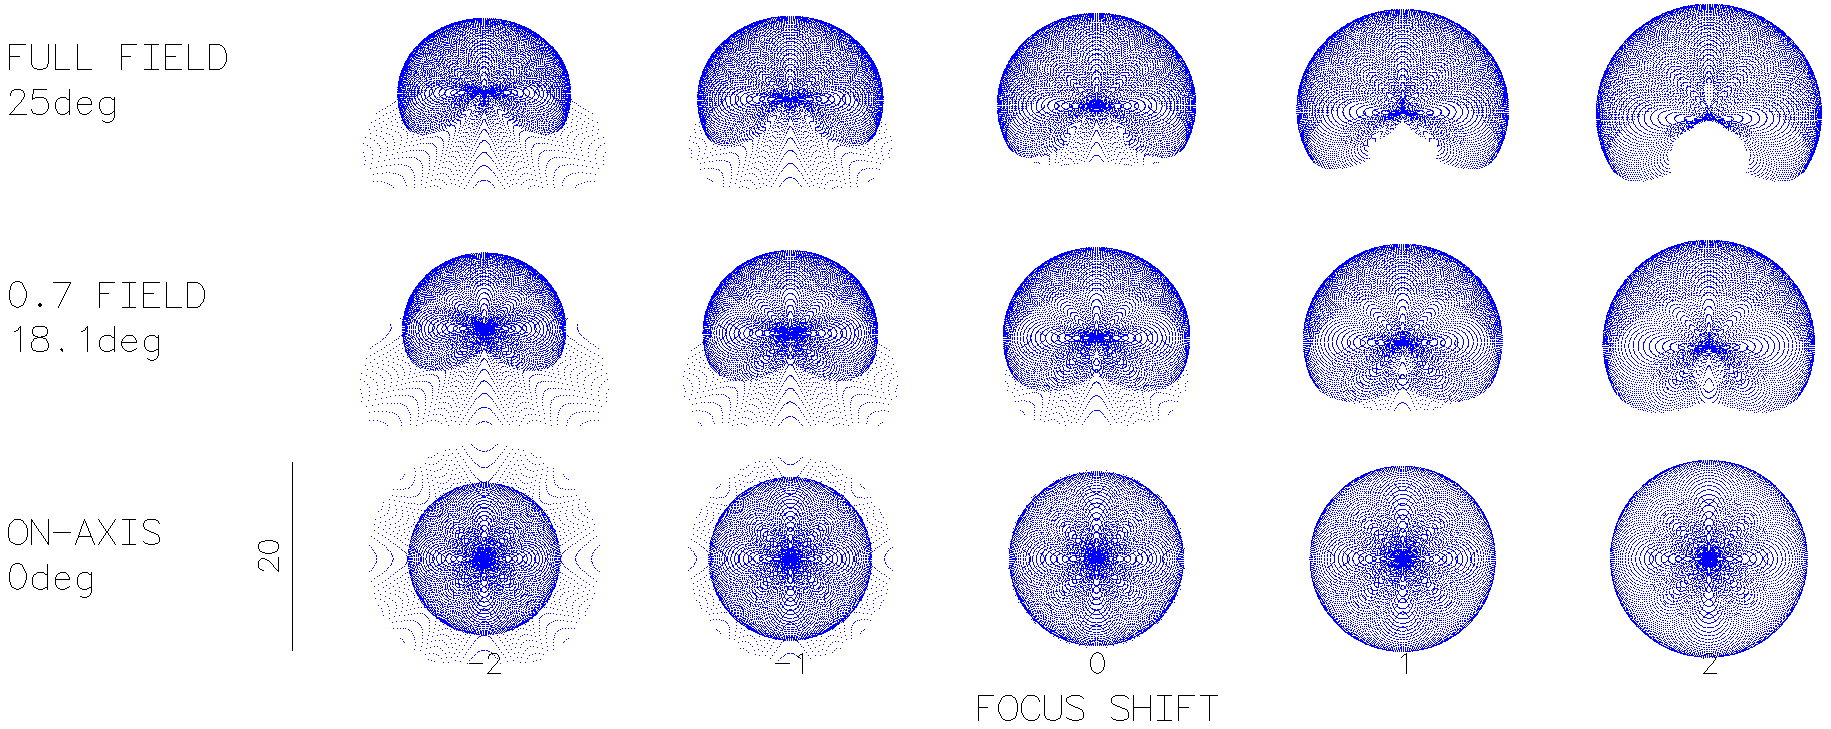
\includegraphics[width=.8\textwidth,trim=0 0 0 0,clip]{Sphere3spot.png}
\caption{\label{fig:spots} Images of light spots on the focal surface of the detector from point light sources taking taking into account the shadow from the mosaic.}
\end{figure}


It is planned to design a compact detector that will have the following characteristics:
Sensitive area of optics (aperture input window) up to 0,1m2;
Mirror diameter up to 80 cm;
Optical system viewing angle $\pm$ 20--25 degrees;
Number of mosaic elements 49 or more SiPM;
The mass of the detector less 10 kg;
The flight height of the detector up to 500 m;
Expected number of events EAS (with $E_0$ = 1--100 PeV) up to 10\,000 for season.

The main element of the new installation will be a segment of seven SiPM Micro FC-60035 SiPMs. The tests of a matrix of seven such segments (49 SiPM) was successfully completed (see figure~\ref{fig:3} left). Each segment was equipped with seven preamplifiers and a temperature sensor to account for the effects of thermal emission. Each SiPM was equipped with a light collector CA10929 Boom-MC-W with angular characteristic $\pm$24 degrees at 50\% effectiveness. In this project, it is planned to modify and adapt the SiPM segment for use in a ultra-wide angle optical system.

The mirror for the detector will be made on the basis of composite materials. The mirror base is made of cellular aluminium This design has sufficient rigidity and low weight.

The detector will use the Schmidt optical system. In this system, the central part of the mirror is not used since it is in the shadow of the photodetector. A hole in the centre of the mirror with a wide-angle lens in it with an aperture of about 100 cm$^2$ will allow registration of the direct CL (see figure~\ref{fig:3} right). Calculations show that for EAS from PCR with 1 PeV energy the CL photons density is around 100 photons per cm$^2$ at a distance of 100 m from the shower axis. Taking into account the SiPM quantum efficiency and losses of optical elements expects to register around 1000 photoelectrons. The estimation of the primary particle mass can use the information on the intensity of the direct CL in addition to the data on the reflected CL.

It is assumed that the EAS from the primary proton should form a light spot different of Fe nuclei at the same primary energy and depth of EAS maximum.

To control the density and transparency of the atmosphere an auxiliary small UAV can be used with pressure, temperature, humidity sensors and laser lidar. The lidar will be used to control the reflection from the snow. Laser control of the atmosphere and reflection from the snow will improve the accuracy of measuring the EAS CL.

The properties of the snow surface play an important role when using the method of reflected CL registration. The results of the show optical properties studies have been repeatedly published by several groups. The simulation results show that in the wavelength range from 300 to 600 nm, the relative reflectance for pure snow is stable within 3\% for the zenith angles of the light incidence from 0 to 80 degrees. From the above mentioned results and the known CL spectral characteristics it can be concluded that the snow surface reflects the CL with minor spectral distortions in the range of zenith angles up to 80 degrees and can be used as a screen for the CL registration.


\begin{figure}[htbp]
\centering % \begin{center}/\end{center} takes some additional vertical space
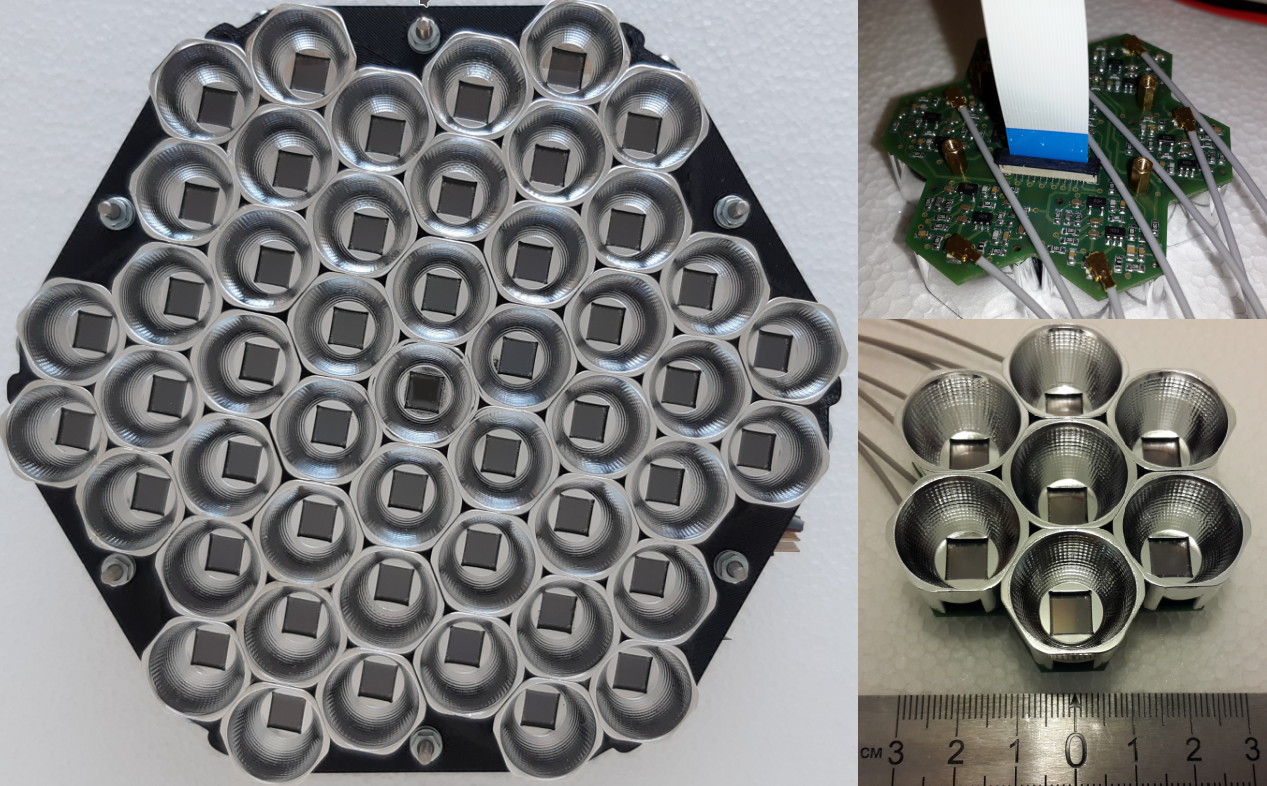
\includegraphics[width=.55\textwidth,trim=0 0 0 0,clip]{mosaic_protype.png}
\qquad
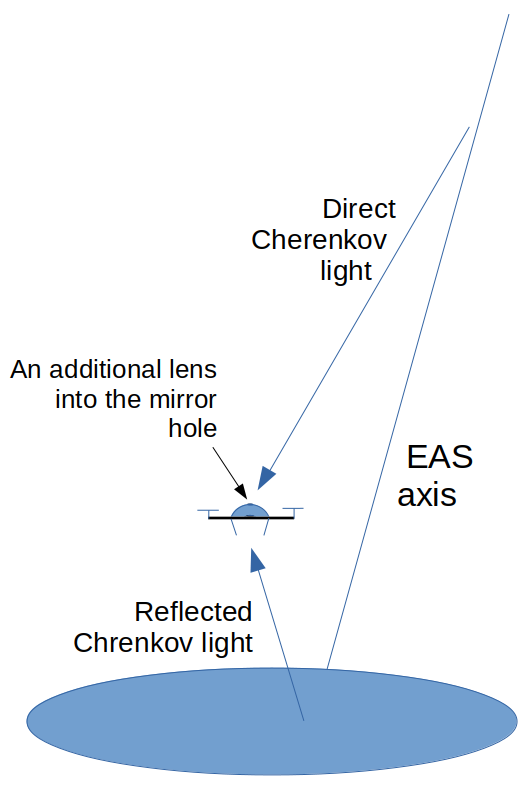
\includegraphics[width=.25\textwidth,origin=c,angle=0]{DirectCL.png}
% "\includegraphics" from the "graphicx" permits to crop (trim+clip)
% and rotate (angle) and image (and much more)
\caption{\label{fig:3} Mosaic prototype (left) and a scheme of direct and reflected Cherenkov light of EAS (right).}
\end{figure}



\section{Hardware and calculation development plan}

План.

\section{The conditions for conducting measurements on a UAV}



%\appendix
%\section{Some title}
%Please always give a title also for appendices.


%\acknowledgments

%This is the most common positions for acknowledgments. A macro is
%available to maintain the same layout and spelling of the heading.

\paragraph{Note added.} This is also a good position for notes added
after the paper has been written.


% We suggest to always provide author, title and journal data:
% in short all the informations that clearly identify a document.

\begin{thebibliography}{99}

\bibitem{1}
D. V. Chernov, R. A. Antonov, T. V. Aulova, E. A. Bonvech, V. I. Galkin, T. A. Dzhatdoev, D. A. Podgrudkov, and T. M. Roganova, \emph{Detection of reflected Cherenkov light from extensive air showers in the SPHERE experiment as a method of studying superhigh energy cosmic rays}, \emph{Physics of Particles and Nuclei} {\bf vol} 46, no. 1, 2015, pp. 60–93.

\bibitem{2}
R. A. Anotov, T. V. Aulova, E. A. Bonvech, D. V. Chernov, T. A. Dzhatdoev, M. Finger, V. I. Galkin, D. A. Podgrudkov, and T. M. Roganova, \emph{Event-by-event study of cr composition with the sphere experiment using the 2013 data}, \emph{Journal of Physics: Conference Series} {\bf vol} 632, no. 012090, 2015, pp. 1–8.

\bibitem{3}
R. A. Antonov, E. A. Bonvech, D. V. Chernov, T. A. Dzhatdoev, V. I. Galkin, D. A. Podgrudkov, and T. M. Roganova, \emph{Spatial and temporal structure of EAS reflected Cherenkov light signal}, \emph{Astroparticle Physics} {\bf vol} 108, 2019, pp. 24–39.


% Please avoid comments such as "For a review'', "For some examples",
% "and references therein" or move them in the text. In general,
% please leave only references in the bibliography and move all
% accessory text in footnotes.

% Also, please have only one work for each \bibitem.


\end{thebibliography}
\end{document}